\section{Robust Regression}
\subsection{Singular values decomposition (SVD)}
After applying the SVD to both $\mathbf X$ and $\mathbf X_{noise}$ data, the Fig.\ref{fig:1_6_a} illustrates the singular values. For the original data $\mathbf X$, there are only three singular values which corresponding to its rank. Due to the randomness and independences of noise, the matrix $\mathbf X_{noise}$ is full rank which has ten singular values. However, there are three significant singular values which represents the dimension of signal subspace. The magnitude of other non-zero singular values are approximate half of the signal singular values, whose difference can be used to detect the signal and noise subspace. Nevertheless, if the noise power is large, it becomes hard to identify the rank of $\mathbf X_{noise}$.
\begin{figure}[htbp]
    \centering
     \begin{subfigure}{0.4\textwidth}
         \centering
         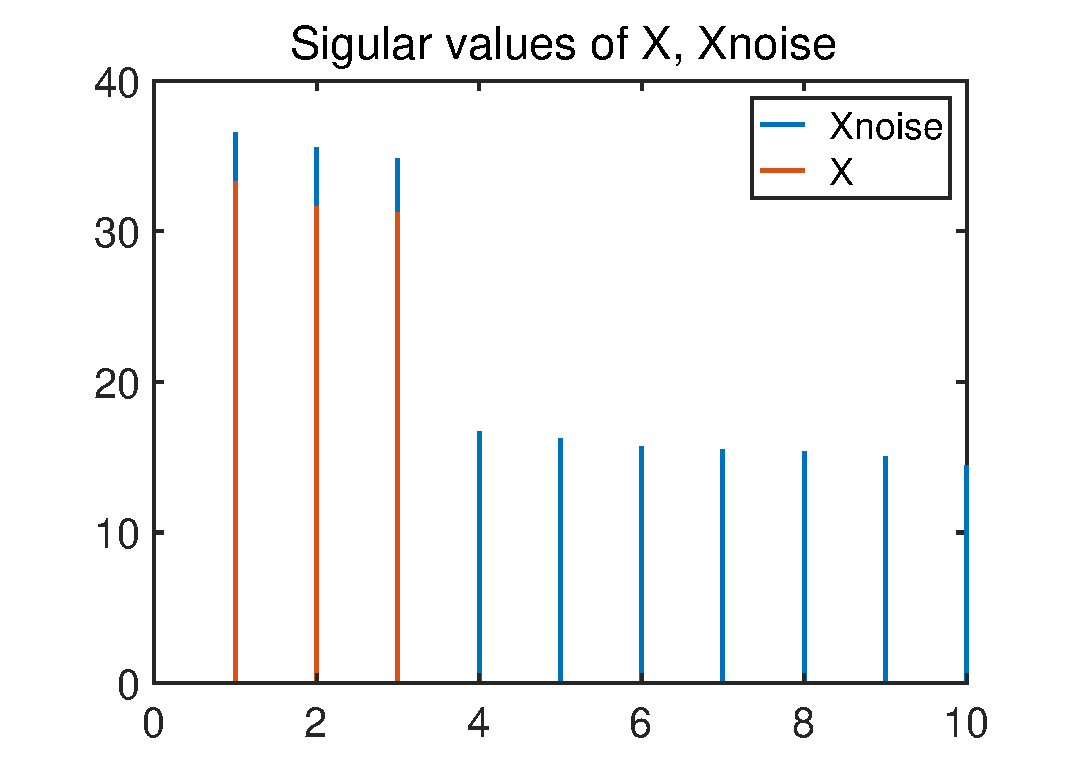
\includegraphics[width=\textwidth]{fig/16/16a1.eps}
     \end{subfigure}
     ~
     \begin{subfigure}{0.4\textwidth}
         \centering
         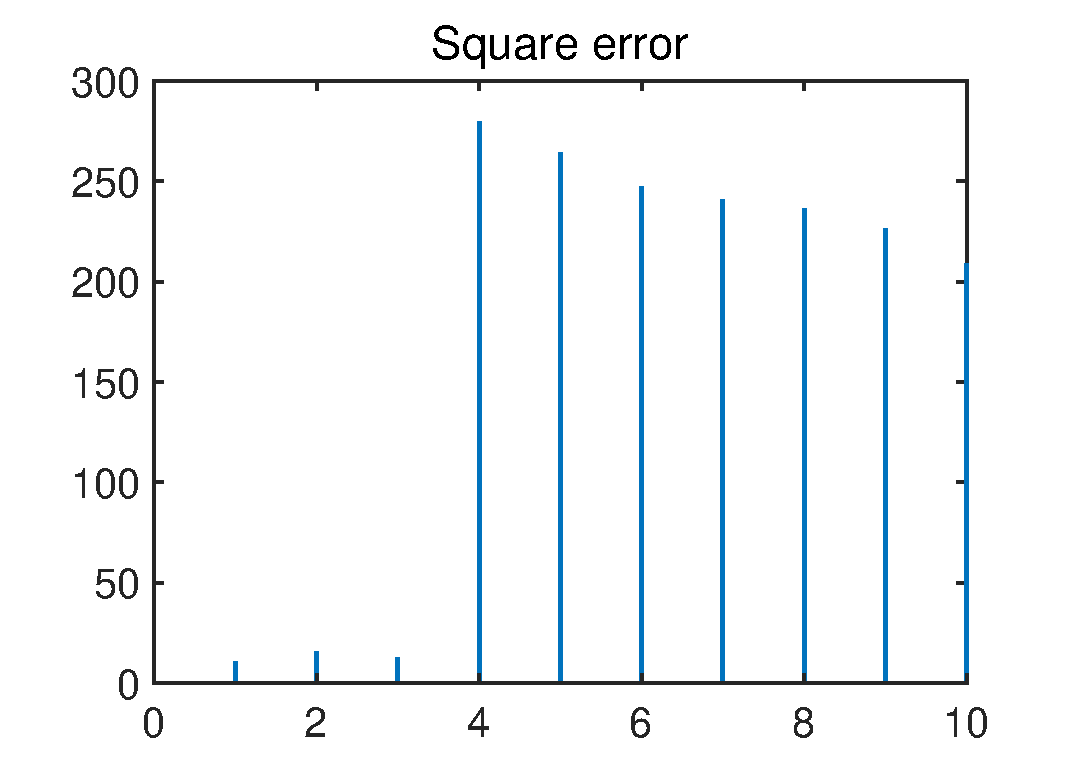
\includegraphics[width=\textwidth]{fig/16/16a2.eps}
     \end{subfigure}
    \caption{SVD of $\mathbf X$ and $\mathbf X_{noise}$}
    \label{fig:1_6_a}
\end{figure}
\subsection{Low rank approximation}
The SVD algorithm could be used to recover the original matrix. Since the noise power is much less than the signal power, the recovered matrix is noiseless if only $k$ significant values are concerned, where $k$ is the rank of the original matrix. Fig.\ref{fig:1_6_b} shows the error between the noise matrix and recovered noiseless matrix. As to the noiseless error curve, when the number of $k$ is equal to the actual rank, the error reaches the bottom point. In this experiment, the minimum point at rank 3 is 27.07, while it is 49.34 of noise error over all rank. Therefore, the rank and the dimension of signal subspace are determined.
\begin{figure}[htbp]
    \centering
    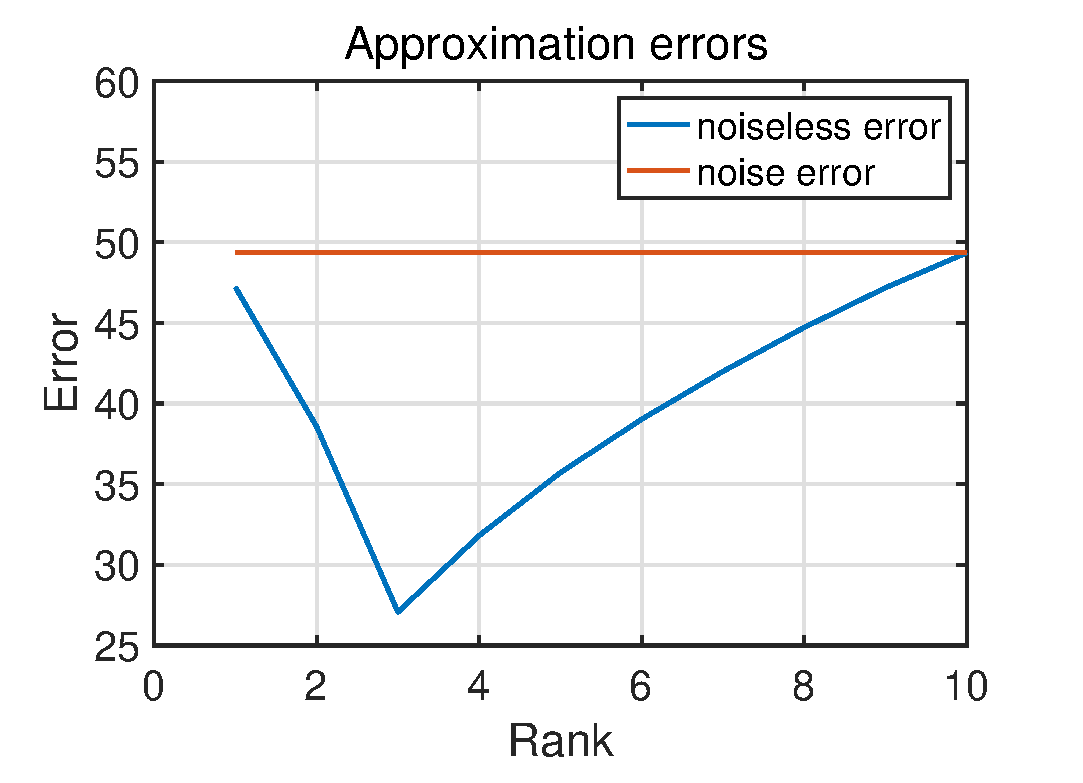
\includegraphics[width=0.4\textwidth]{fig/16/16b.eps}
    \caption{Error in low rank approximation}
    \label{fig:1_6_b}
\end{figure}
\subsection{OLS vs PCR}
The parameter matrix $\mathbf B$ is calculated based on the OLS and PCR method. Meanwhile, the square error between the actual $\mathbf Y$ and estimated output on training and testing data are illustrated in Fig.\ref{fig:1_6_c}. When the number of significant components $k$ is larger than 3, the PCR has the same performance with the OLS method. However, when testing the parameter matrix via $\mathbf X_{test}$, the estimated error of the PCR increases with $k<3$, while the error of OLS decreases.
\begin{figure}[htbp]
     \centering
     \begin{subfigure}{0.4\textwidth}
         \centering
         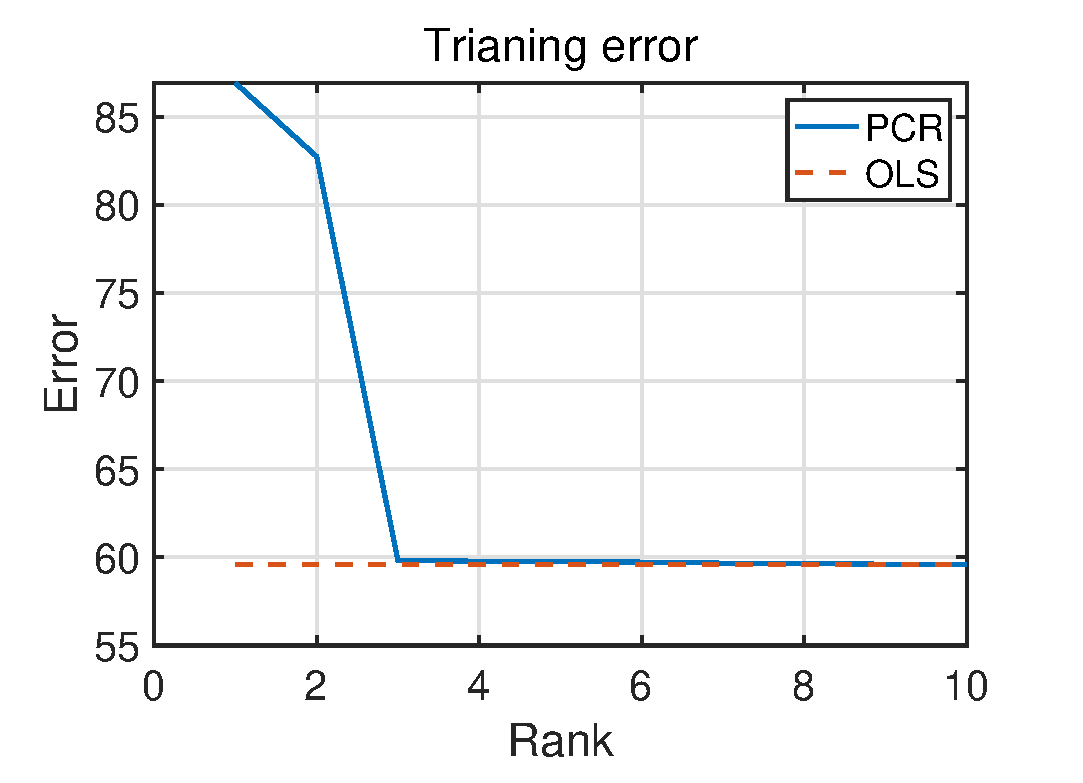
\includegraphics[width=\textwidth]{fig/16/16c1.eps}
     \end{subfigure}
     ~
     \begin{subfigure}{0.4\textwidth}
         \centering
         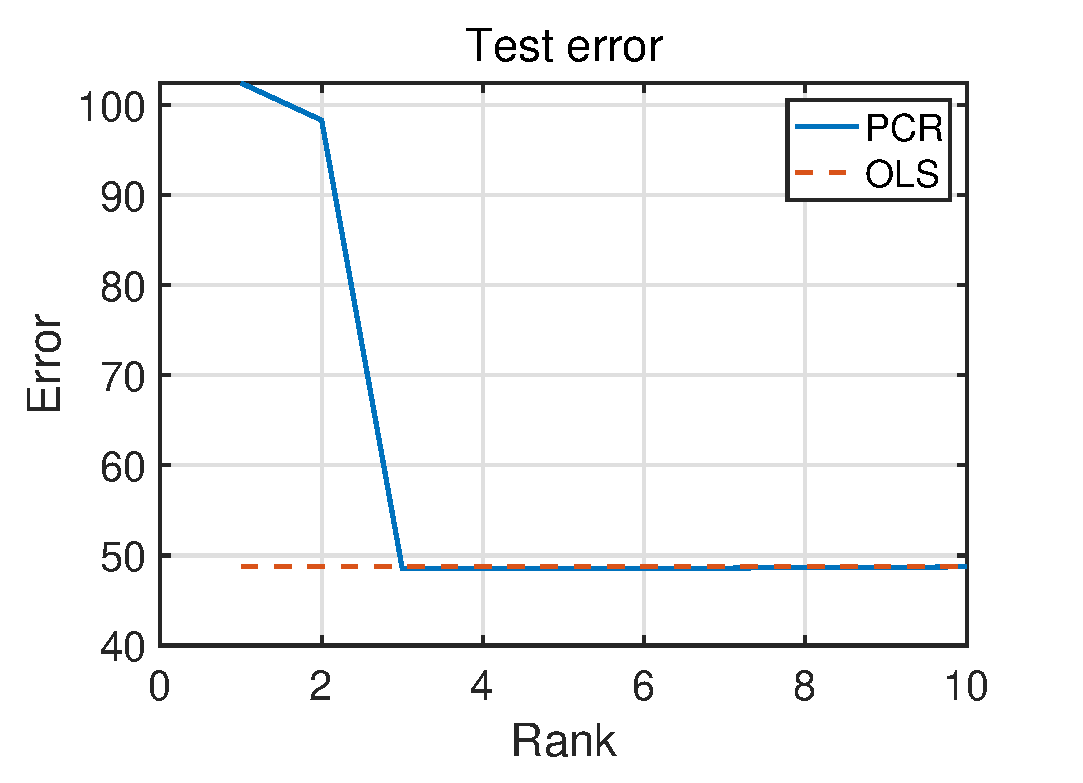
\includegraphics[width=\textwidth]{fig/16/16c2.eps}
     \end{subfigure}
        \caption{Training and testing error of OLS \& PCR}
        \label{fig:1_6_c}
\end{figure}
\subsection{Realisations of OLS and PCR}
Totally 50 realisations were simulated by OLS and PCR methods and its average error with test data are plotted in Fig.\ref{fig:1_6_d}. Compared with the testing error shown in Fig\ref{fig:1_6_c}, the average errors of both PCR and OLS algorithms are reduced to a large extent. The largest error of PCR is reduced from 85 to 65, while the OLS decreases to 37.81.
\vspace*{3in}
\begin{figure}[t!]
    \centering
    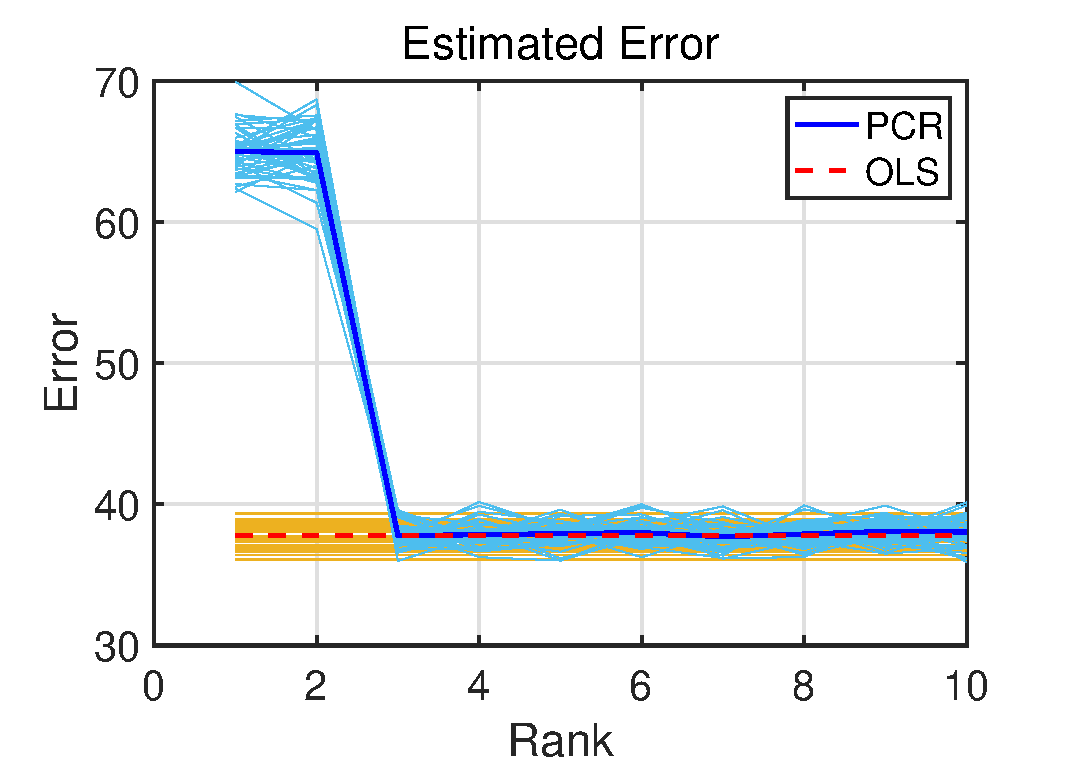
\includegraphics[width=0.4\textwidth]{fig/16/16d.eps}
    \caption{Estimated error of realisations}
    \label{fig:1_6_d}
\end{figure}


